%! Author = mboehme
%! Date = 01.03.2023

\newpage
\section{Ergebnis}\label{sec:ergebnis}
Das Ergebnis sieht wie folgt aus:
\subsection{Visuelle Darstellung}\label{subsec:visuelle-darstellung}
%include two images
\par\vspace{1cm}
    \centering
    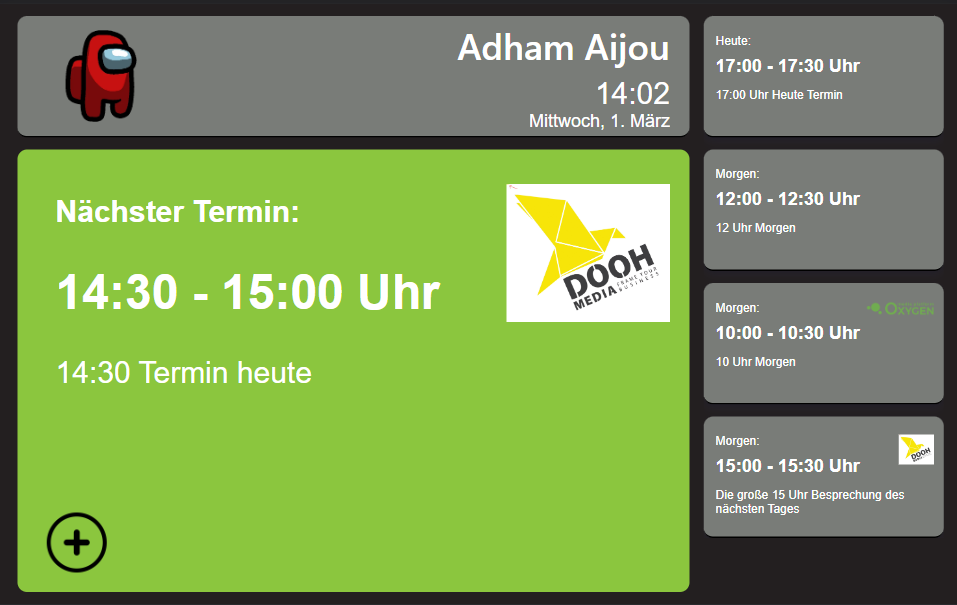
\includegraphics[width=0.8\textwidth]{Bilder/Ergebnis}
    \caption{Ergebnis mit nächstem anstehenden Termin}
    \label{fig:Ergebnis mit nächstem anstehenden Termin}
\par\vspace{1cm}
\raggedright
\par\vspace{1cm}
    \centering
    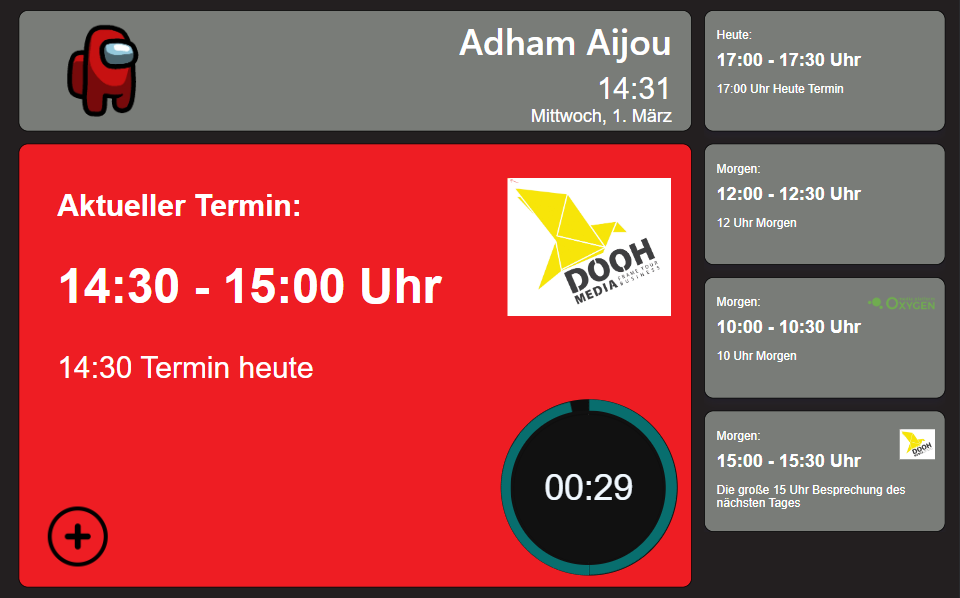
\includegraphics[width=0.8\textwidth]{Bilder/Ergebnis_LaufenderTermin}
    \caption{Ergebnis mit laufendem Termin}
    \label{fig:Ergebnis mit laufendem Termin}
\par\vspace{1cm}
\raggedright
\newline
Oben links im Bild, das Bild des kleinen roten Charakters, sieht man das Logo des Gastgebers des nächsten, beziehungsweise jetzigen, Termins.
Solch ein Logo kann dargestellt werden, indem beim Erstellen des Termins, außerhalb des Tablets, bei Outlook beispielsweise, ein Bild hochgeladen wird, welches im Betreff eine bestimmte Bezeichnung enthält, die hier aus Sicherheitsgründen nicht genannt werden kann.
\newline
Die anderen Logos, sind alle Logos vom Gast des Termins.
Diese Logos können an alle Geräte gleichzeitig versendet werden, indem ein spezieller Termin erstellt wird, der nur für die Logos gedacht ist und eine einzigarte ID, sowie Befehle enthält, die dann das Bild, inklusive Firmennamen, in einer lokalen Datenbank abspeichert.
Diese Logos können hinzugefügt, gelöscht oder aktualisiert werden.
Aus Sicherheitsgründen werden die genaueren Befehle der Schnittstelle hier nicht genannt.
\newline
Es wird immer nur der erste Gast angezeigt, da das so vom Kunden gewünscht wurde.
\newline
Die Uhrzeit wird, immer, in der Zeitzone des Tablets angezeigt.
\newline
\newline
Hier sieht man nochmal das Menü, wo ein Termin gebucht werden kann, welches durch das Drücken des Plus-Symbols aufgerufen wird:
\par\vspace{1cm}
    \centering
    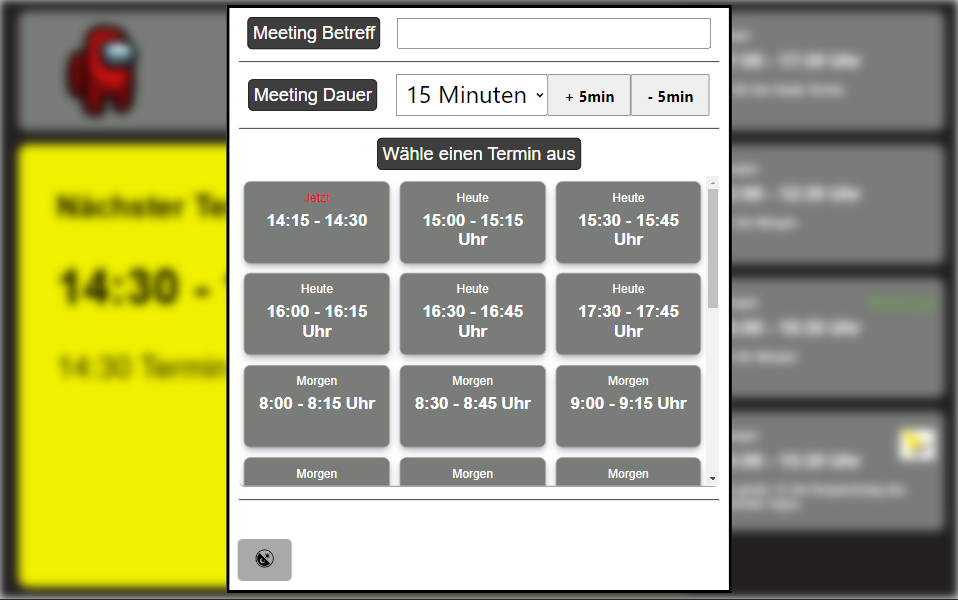
\includegraphics[width=0.8\textwidth]{Bilder/Ergebnis_TerminErstellen_Menue}
    \caption{Menü}
    \label{fig:Menue}
\par\vspace{1cm}
\raggedright
Wie man sieht, ist beispielsweise die selbsterstellte Option \("\)Jetzt\("\) deaktiviert, da das Ende des hypothetischen Termins innerhalb von 15 Minuten vom nächsten anstehenden Termin beginnt.
Diese Pufferzeit wurde so mit dem Kunden abgesprochen.
Auf die anderen Optionen hat man hier wenig Einfluss, da sie von den Einstellungen des Kalenders, des jeweiligen Nutzers, abhängen und es somit in der Verantwortung des Nutzers liegt, diese zu ändern.
\newline
\newline
Hier die normale Ansicht nochmal, aber im light-Modus:
\par\vspace{1cm}
    \centering
    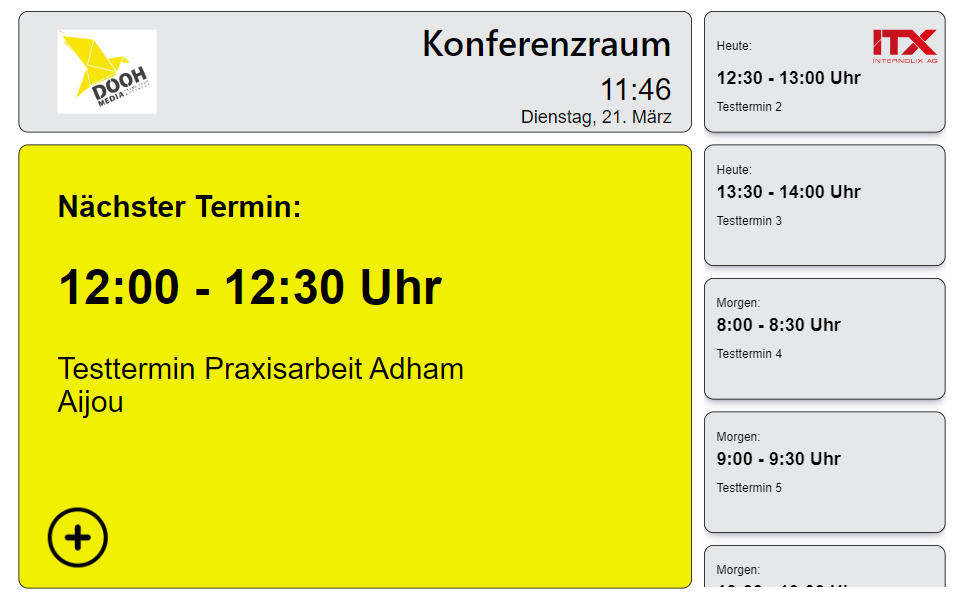
\includegraphics[width=0.8\textwidth]{Bilder/Ergebnis_lightMode}
    \caption{Prototyp im light-Modus}
    \label{fig:PrototypLight}
\par\vspace{1cm}
\raggedright
\newline
\newline
\subsection{Performance}\label{subsec:performance}
Die Performance einer SPA zu messen ist nicht ganz einfach.
Auch die gängige Total-Blocking-Time Messung ist nicht zwingend sinnvoll, da die Anwendung ja nicht blockiert, sondern nur die Daten vom Server lädt und danach die Nutzung der Anwendung möglich ist.
Daher wurden manuell einige Tests durchgeführt, um die Performance zu messen.
\newline
\newline
\subsubsection{Test 1}\label{subsubsec:test-1}
\newline
\newline
Wie lange braucht die Anwendung, um nach einem Klick auf den Button \("\)+\("\) das Terminerstellungs-Menü zu öffnen?
Diese Frage wurde gemessen, indem der Event-Listener auf den Button \("\)+\("\) registriert wurde und die Zeit gemessen wurde, die vergeht, bis der Event-Listener aufgerufen wurde und das Menü dargestellt wurde.
Es dauert im Durchschnitt 2ms, bis das Menü angezeigt wird.
\newline
\newline
\subsubsection{Test 2}\label{subsubsec:test-2}
\newline
\newline
Wie viele Bilder pro Sekunde zeigt die Anwendung durchschnittlich an?
Dies wurde mithilfe von LightHouse gemessen.
Die Anwendung zeigt durchschnittlich 60 Bilder pro Sekunde an.
\newline
\newline
\subsubsection{Test 3}\label{subsubsec:test-3}
\newline
\newline
Wie oft, kann die Anwendung theoretisch und praktisch pro Sekunde aktualisiert werden?
Für jede Kombination aus Azure App und E-Mail-Adresse, dürfen 10000 Anfragen pro 10 Minuten gemacht werden.
Dies sind 16,6 Anfragen pro Sekunde.
Praktisch wurden eine bis drei Anfragen, je nach Bedarf, pro drei Sekunden gemacht.
Pro Sekunde wären das also 0,33 bis 1 Anfragen.
Einerseits ist das schnell genug für die Anwendung und gibt den langsamen Geräten, genug Zeit, die Anwendung zu aktualisieren, andererseits hat man so genug Anfragen übrig, falls jemand sein Konto mit mehreren Geräten benutzt oder dies in Kombinationen mit anderen Applikationen verwendet.
Sollte dieses Limit überschritten werden, verlangsamt Microsoft die Anzahl an neuen Antworten auf die Anfragen.
Da Microsoft sowieso auch Zeit benötigt, um die Anfragen zu bearbeiten und die neuen Daten bei sich zu verarbeiten, würde man den Unterschied nicht merken.
Der Bottleneck \
\newline
\newline
